\documentclass[12pt,a4paper]{article}
\usepackage[utf8]{inputenc}
\usepackage[sfdefault]{ClearSans}
\usepackage[T1]{fontenc}
\usepackage[left=35mm,right=20mm,top=25mm,bottom=25mm]{geometry}
\usepackage[czech]{babel}
\usepackage{titling}
\usepackage{graphicx}
\usepackage{caption}
\usepackage[list=true]{subcaption}
\usepackage{acronym}
\usepackage{setspace}
\usepackage{indentfirst}
\usepackage{hyperref}
\usepackage{listings}
\usepackage{tabularx}

\newcommand{\subtitle}[1]{%
	\posttitle{%
		\par\end{center}
		\begin{center}\large#1\end{center}
		\vskip0.5em}%
}

\newcommand*\wildcard[2][5cm]{\vspace*{2cm}\parbox{#1}{\centering\hrulefill\par#2\par}}

\graphicspath{ {./img/} }

%\onehalfspacing
\setlength{\parindent}{2em}
\setlength{\parskip}{0.1em}
\linespread{1.5}

\title{PlantHub}
\subtitle{MATURITNÍ ZKOUŠKA }
\author{Filip Sikora, Jakub Vantuch}
\date{}

\begin{document}

\begin{titlepage}
	\noindent
\includegraphics[width=\linewidth]{header.png}
	%\vspace{0.1cm} \\
	\begin{center}
		\vspace*{0.2cm}
		\Huge\textbf{MATURITNÍ ZKOUŠKA}
		\vspace*{1cm} \\
		\large \emph{PRAKTICKÁ ZKOUŠKA Z ODBORNÝCH PŘEDMĚTŮ}
		\vspace*{1cm} \\
		\Large Téma č. 4 \\
		\vspace*{1cm}
		\Large Zavlažovací systém PlantHub \\
		\vspace*{1.3cm}
		%\vfill
		\normalsize
	\end{center}
	\begin{tabularx}{\textwidth}{l@{\hskip 0.5cm}XXl}
		Obor vzdělání:        & \multicolumn{3}{c}{\textbf{18 – 20 –
		M/01
		Informační technologie}}
		\\[10pt]
		Třída:                & \textbf{4. IT}
		                      &
		Autor práce:          & \textbf{Jakub Vantuch}
		\\[10pt]
		Školní rok:           & \textbf{2021/22}
		                      &
		Vedoucí učitel práce: &
		\textbf{Ing. Jiří Sumbal}
		\vspace*{2cm}
	\end{tabularx}
	„Prohlašuji, že jsem tuto práci vypracoval samostatně a použil jsem
	literárních
	pramenů a informací, které cituji a uvádím v seznamu použité literatury
	a
	dalších zdrojů informací.“

	\begin{tabularx}{\textwidth}{l@{\hskip 0.5cm}XXl}
		\\[10pt]
		V Frýdku-Místku, dne:             & \textbf{\dotfill}
		                                  &
		\textbf{\dotfill} & podpis
	\end{tabularx}
\end{titlepage}

\clearpage

\section*{Anotace}

PlantHub je automatický zavlažovací systém s \ac{WUI}.
Jádrem našeho systému je mikropočítač \ac{RPi} s procesorovou architekturou
\ac{ARM},
\ac{GPIO} a možností připojení pomocí ethernetu.
Vybrali jsme si jej, protože kombinuje malou velikost a vyšší výpočetní sílu
než Arduino. Musí totiž zvládnout řídit všechny senzory, ukládat data do
databáze a zároveň hostuje i samotnou webovou aplikaci. Systém PlantHub dále
získává informace o teplotě, vlhkosti a tlaku vzduchu a promítá je ve svém
\ac{WUI}. Ve stejné chvíli naměřená data ukládá do databáze v periodě 4
hodin. Jelikož voda časem z nádrže dojde systém PlantHub snímá stav hladiny
vody v nádrži a včas upozorní, že je třeba doplnit vodu.

\section*{Klíčová slova}

zavlažování; automatizace; statistika; živě; RaspberryPi; uživatelské rozhraní

\clearpage

\tableofcontents

\clearpage

\section{Úvod}

Mým cílem je návrh, sestavení a naprogramování automatického zavlažovacího
systému s názvem PlantHub. Systém se skládá z řídící jednotky (stanice),
senzorů, čerpadla, nádrže a \ac{WUI}. Tato stanice pravidelně snímá data ze
senzorů
měřících
teplotu a vlhkost vzduchu, vlhkost půdy a stav hladiny v nádrži, z té pak
stanice přečerpává vodu pomocí čerpadla spouštěného tranzistorem. Naměřená
data
se posílají živě pomocí \ac{REST} \ac{API} prostřednictvím
protokolu HTTP do \ac{WUI}. Samostně se poté v periodě čtyř hodin ukládají do
PostgreSQL databáze běžící v docker
containeru. Docker container si můžeme představit jako jednodušší a lépe
škálovatelnou verzi
virtualizace. Uložená data se vykreslí do
statistik
změn teploty a vlhkosti vzduchu, vlhkosti půdy a počtů zavlažování v časovém
rozsahu zobrazitelných v dashboardu \ac{WUI}. Pro načtení historických dat z
databáze
používáme \ac{GraphQL} \ac{API}, jelikož nabízí šetrnější přístup k datům,
vybráním pouze
těch záznamů z tabulky, které opravdu využíváme. V případě nedostupnosti
serveru by se ve \ac{WUI} měla pořád načítat živě naměřená data z \ac{REST}
\ac{API}. Přístup
k naměřeným datům a
\ac{WUI} má pouze
uživatel lokální
sítě, do které je planthub připojen pomocí ethernet kabelu. Pro správnou funkci
stanice je tedy zapotřebí router s přístupem k internetu a DHCP serverem.

Ve \ac{WUI} hostovaném na naší stanici, a sestavém pomocí javascriptového
frameworku
React.js, CSS frameworku
Tailwind a programovacího jazyku Typescript, který je supersetem javascriptu,
podporujícím volitelné statické typování, má uživatel
možnost zobrazení statistik jak živě naměřených dat tak dat historických v
nastavitelných grafech dashboardu. \ac{WUI} také nabízí manuální kontrolu nad
čerpadlem s časovačem začátku zavlažování a restartem hlavního programu.
Nastavitelné je jak \ac{WUI} tak i samotné faktory zavlažování jako je limit
vlhkosti
půdy, doba zavlažování nebo limit hladiny vody.

Jednotlivé součásti a moduly stanice jsme vybrali podle finanční dostupnosti a
adekvátních technických
požadavků na přesnost měření.
Zapojení těchto modulů do obvodu jsme prvně provedli ve webové aplikaci
EasyEDA, která nabízí jednoduché prostředky pro návrh technických
schémat. Tento obvod jsme poté v testovací verzi postavili na nepájivém
poli a ve finální verzi navrhli a objednali vlastní \ac{PCB}. Pro ochranu naší
stanice jsme v open-source programu FreeCad navrhli model krytu, který jsme
následně vytiskli na 3D tiskárně. Vymstila se nám však nepřesnost rozměrů krytu
a při vkládání stanice do krytu se nám podařilo zlomit SD kartu s operačním
systémem, daty a nasazenými programy. Po reinstalaci operačního systému jsme
opravili rozměry vytvořeného modelu krytu a
vytiskli kryt podruhé, tentokrát ve správných rozměrech.

Hlavní program jsme v prvotní verzi psali ve vysokoúrovňovém programovacím
jazyce Python, od kterého jsme nakonec upustili kvůli vysokým technickým
nárokům. Naše rozhodnutí nás nakonec dovedlo k jazyku
Go vytvořeného Googlem a určeného pro concurrency, rychlou kompilaci i průběh
programu, backend webových aplikací a mnoho
další funkcionality. Tento jazyk se nám zalíbil natolik že jsme se v něm
rozhodli
udělat jak \ac{API},
databázové funkce tak i hlavní program. Program je rozdělen na několik sekvencí
z toho hlavní jsou měřící sekvence kde se každou sekundu provádí měření dat ze
senzorů a následné odesílání na \ac{REST} \ac{API} webové aplikace a channely
vytvořené
pro komunikaci mezi go rutinama a sekvence controlleru, která pomocí snímání
dat z databáze určuje jestli se jedná o první spuštění PlantHubu, a podle toho
určí jestli se spustí incializační sekvence nebo sekvence zavlažování.

\clearpage

\section{Seznam zkratek a pojmů}

\begin{acronym}
	\acro{WUI}{Webové uživatelské rozhraní}
	\acro{API}{Application programming interface}
	\acro{REST}{Representaion programming interface}
	\acro{GraphQL}{Graph query languge}
	\acro{PCB}{Printed circuit board}
	\acro{RPi}{Raspberry Pi}
	\acro{CPU}{Central Processing Unit}
	\acro{ARM}{Advanced RISC Machines}
	\acro{GPIO}{General-purpose input/output}
	\acro{ADC}{Analogově digitální převodník}
	\acro{DHT11}{Digital humidity temperature v.11}
	\acro{HC-SR04}{Ultrasonický senzor vzdálenosti}
	\acro{LED}{Light Emitting Diode}
	\acro{SAR}{Successive-approximation}
	\acro{PETG}{Polyethylene terephthalate glycol filament}
	\acro{LSB}{Least significant bit}
	\acro{CLR}{Common Language Runtime}
	\acro{JVM}{Java virtual machine}
\end{acronym}

\clearpage

\section{Hardware}

Potřebujeme vyvinout vhodné pouzdro pro naše Raspberry, abychom ochránili
citlivé elektronické součástky a ve stejné chvíli měli možnost jednoduše
vyjmout stanici z krytu. Budeme ho tisknout na 3D tiskárně pevným \ac{PETG}
filamentem. K
zavlažování je potřeba postavit i nádrž na vodu, ze které bude naše čerpadlo
přečerpávat vodu k zavlažování, proto jsme se rozhodli pro nádobu s co
nejvetším objemem a postavili ji z upraveného 5L soudku.

\subsection{Senzory}

\subsubsection{Senzor teploty a vlhkosti vzduchu DHT11}

Senzor \ac{DHT11} se skládá z jednotky pro měření teploty, jednotky pro měření
vlhkosti a převodníku.

Teplotu měří senzor thermistorem. Thermistor je keramický polovodič, který
zmenšuje svou rezistivitu, když se okolní teplota zvýší.

Vlhkost měří senzor na základě rezistivity substrátu umístěného mezi dvěma
elektrodami. Tento substrát zachytává vlhkost a vytváří tak vodivé prostředí

\subsubsection{Senzor vlhkosti půdy}

Jedná se o kapacitní senzor, ten se skládá ze dvou vodivých desek a převodníku.
Čidlo funguje na způsob kapacitoru avšak jeho kapacita je ovlivněna vlhkostí,
která ovlivňuje dielektrikum mezi dvěma deskami.

\subsubsection{Analogově digitální převodník MCP3008}

\ac{RPi} má v rámci \ac{GPIO} pouze digitální vstupy, protože je ale senzor
vlhkosti půdy
analogový museli jsme použít \ac{ADC}. Přemapujeme tedy analogový
signál
do
osmi různých digitálních hodnot, kterým se také říká 3bitové rozlišení, to
definuje tu nejmenší hodnotu změny, který převodník dokáže rozlišit, této
hodnotě se říká \ac{LSB}. \ac{ADC} poté pomocí \ac{SAR}
definuje adresu v binárním podání srozumitelným pro digitální vstup.

% \begin{figure}[h]
% 	\centering
% 	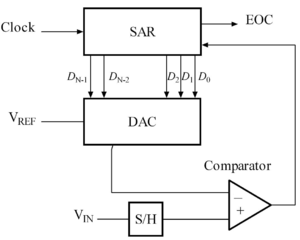
\includegraphics[width=8cm]{sar_adc.png}
% 	\caption{\ac{SAR}}
% \end{figure}

\subsubsection{Ultrasonický senzor HC-SR04}

\ac{HC-SR04} vydává zvukové vibrace na vysoké frekvenci, neslyšitelné pro
lidské
ucho. Poté čeká, až se zvuk odrazí zpět, a vypočítá vzdálenost na základě času
měřeného od vysílání zvukové vlny k zpětnému přijmutí

Všechny naměřené údaje jsou v převodníku senzoru přepočítány na jednotky dané
veličiny a odeslány analogovým signálem do řídící jednotky.

\subsubsection{Čerpadlo}

Naše zvolené ponorné mini čerpadlo eses se skládá z DC motoru, na němž je
upevněna centrifuga pro
čerpání vody a vlastního pouzdra, z kterého vede otvor pro napojení odtokové
hadičky. Čerpadlo je připojeno na zdroj napětí 5V a zem.

\subsubsection{Tranzistor 2N2222}

Protože samotný signální pin neposkytuje dostatečné napětí pro chod čerpadla
ovládáme jej tranzistorem 2N2222. Tento tranzistor je bipolární
Negative-Positive-Negative tranzistor, to znamená že jeho polarita je nastavená
tak aby na kolektoru přijímal pozitivní napětí. Díky našemu vyměnitelnému
připojení modulů je
možné čerpadlo vyměnit a přívodný kabel používat jako spouštěč čerpadla
jakéhokoliv výkonu a nároků na zdroj.

\subsection{Architektura ARM}

\ac{ARM} je nejnovější \ac{CPU} architektura. Využívají ji všechny moderní
chytré
telefony, zařízení s operačním systémem Android i Apple produkty. Dnes už mají
\ac{ARM} procesory zařízení s Windows nebo MacOS.\@

% \ac{ARM} je založen na RISC (Reduced Instruction Set Computing), tyto procesory jsou designované na 

\clearpage

\section{Návrh obvodu a plošného spoje}

Testovací verzi našeho obvodu jsme postavili na nepájivém kontaktním poli,
které jsme používali pouze v testovací verzi. Jakmile jsme měli vše plně
odzkoušeno a plně otestováno přešli jsme na profesionálnější řešení.
Což tedy v druhé fázi znamenalo sestrojit a nechat vytisknout náš vlastní obvod
přepracovaného schématu \ac{PCB} a vytisknutého společnosti JLCPCB na naše
vlastní
náklady.

\begin{figure}[h]
	\centering
	\begin{subfigure}[b]{0.4\linewidth}
		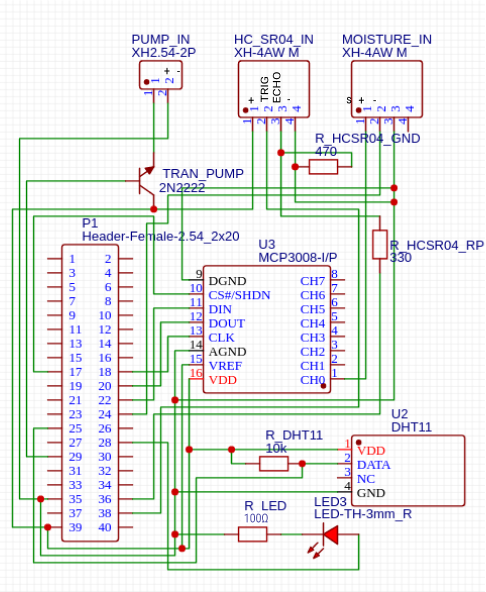
\includegraphics[width=\linewidth]{pcb.png}
		\caption{Diagram \ac{PCB}}
	\end{subfigure}
	\begin{subfigure}[b]{0.4\linewidth}
		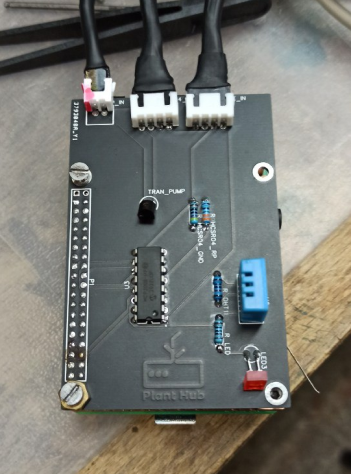
\includegraphics[width=\linewidth]{planthub.png}
		\caption{PlantHub \ac{PCB} se senzory}
	\end{subfigure}
	\caption{}
\end{figure}

\clearpage

\section{Fyzická realizace}

% předělat na fotku celého planthubu

\begin{figure}[h]
	\centering
	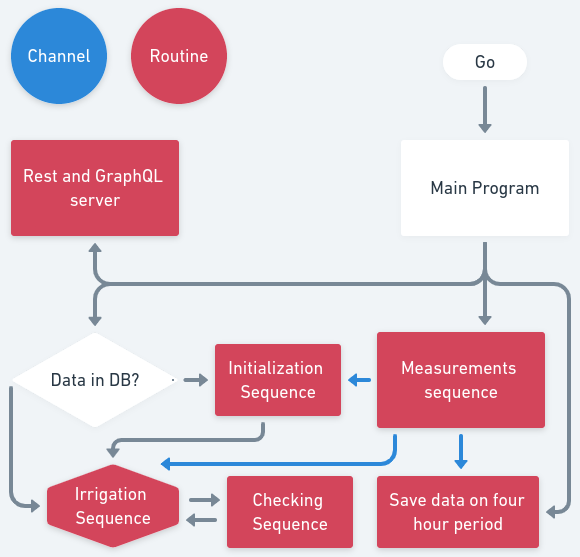
\includegraphics[width=0.72\linewidth]{go.png}
	\caption{Fyzická realizace}
\end{figure}

\clearpage

\section{Hlavní program}

\subsection{Postup práce}

Náš hlavní program pro zavlažování a komunikaci s databází a \ac{WUI}
jsme začali psát ve vysokoúrovňovém programovacím jazyce Python. Od toho jsme
ale nakonec upustili kvůli horší výkonu, a tak jsme program přepsali v
programovacím jazyku Go.

\begin{figure}[h]
	\centering
	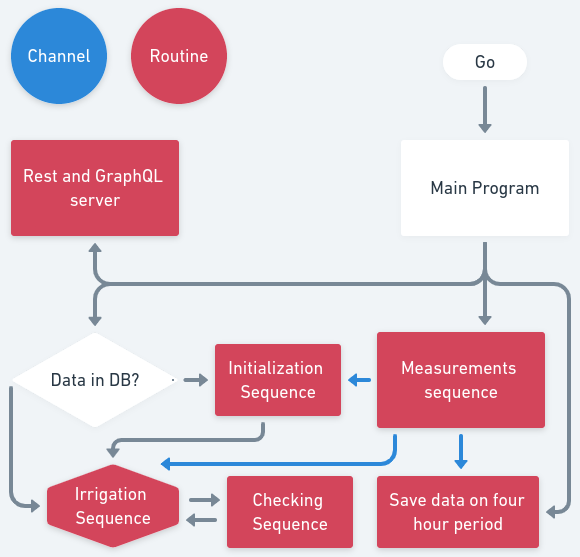
\includegraphics[width=0.72\linewidth]{go.png}
	\caption{Vývojový diagram programu}
\end{figure}

\subsection{Fáze programu}

Fáze programu se spouštějí buďto v samostatné go rutině a komunikují spolu
pomocí channelů nebo na základě podmínek kde se po splnění požadavků ukončí.

\subsubsection{Měření}

Senzor vlhkosti půdy a \ac{DHT11} průběžně posílají naměřená data do \ac{RPi},
kde se
ukládají do databáze. Jestliže naměřené hodnoty překročí limitní hodnoty,
\ac{RPi}
pošle signál pro otevření tranzistoru což spustí čerpadlo.

\subsubsection{Periodické ukládání dat}

V samostatné rutině běží funkce pro ukládání naměřených dat v periodě 4 hodin.
Naměřená data jsou následně statisticky zobrazena v \ac{WUI}.

\subsubsection{Controller}

Po spuštění měřící sekvence a sekvence periodického ukládání dat se spustí
buďto incializační sekvence a nebo zavlažovací sekvence podle toho jestli jsou
v databázi data nastavení, nastavovaná ve \ac{WUI}. Pokud data nejsou tak
program
čeká na uložení dat z \ac{WUI} a \ac{LED} dioda bliká dvakrát po sobě dokud
data
nejsou
dostupná, pokud ano spustí se zavlažovací sekvence, načtou se limitní data z
databáze a v periodě 1 sekundy se budou číst data o vlhkosti půdy.

\subsubsection{Inicializace}

Půda musí být ze začátku suchá. Senzor vlhkosti půdy zasuneme co nejhlouběji do
půdy. \ac{RPi} bude chvíli sbírat data a pak je zprůměruje do hodnoty, která
bude
sloužit jako limit pro spuštění čerpadla.

V \ac{WUI} jde navíc ještě manuálně nastavit hranice vlhkosti půdy pro spuštění
čerpadla.

Nastavit se dá také množství vody, které bude přečerpáno při jednom spuštění a
jaká je hranice pro přijatelnou výšku hladiny vody v nádrži. Pokud nejsou tyto
hodnoty uvedeny čerpadlo bude vodu přečerpávat, dokud se nezmění hodnota
kapacitního čidla pro měření vlhkosti půdy a \ac{HC-SR04} použije výchozí
nastavení.

\subsubsection{Zavlažování}

Čerpadlo začne čerpat vodu a zavlažovat rostlinu. Voda se čerpá tak dlouho,
dokud senzor vlhkosti půdy nezmění svou hodnotu nebo dokud není vyčerpán limit
přečerpané vody na jedno spuštění.

\subsubsection{Kontrola}

Po ukončení přečerpávání se spustí \ac{HC-SR04} a změří výšku hladiny vody.
Naměřená
data poté odešle do \ac{RPi} kde se uloží do databáze. Pokud bude naměřená
hodnota
nižší, než je limitní hodnota, začne blikat \ac{LED} a \ac{RPi} odešle
upozornění o
doplnění nádrže do \ac{WUI}. Jakmile bude hladina doplněna, signalizace se
vypne.

\subsubsection{Ukládání dat}

Náš systém ukládá zvlášť periodicky naměřená data a data naměřená před
zavlažováním, dále ukládá nastavení jak pro limity k zavlažování, tak pro
\ac{WUI}.

\subsection{Go}

Go je open-source programovací jazyk, který byl vytvořen společností Google v
roce 2009. Je to stále relativně nový programovací jazyk, který se nevyvinul z
jiných jazyků jako C\# a Java. Go ignoruje teorii o programovacích jazycích.
Místo toho aby se zaměřoval na akademické teorie, se zaměřuje na reálné
praktiky používané pro vývoj next-gen v cloudových, distribuovaných a
souběžných aplikacích.

Jazyk Go je staticky typovaný a využívá garbage collector, jedná se o
kompilovaný programovací jazyk, který své binární soubory kompiluje pro každou
platformu. Dá se zařadit do skupiny C jazyků na základě jeho základního
syntaxe. Go poskytuje expresivní syntax s jednoduchým typovým systémem a má
vestavěné nástroje pro paralelní programování. Výkon Go je srovnatelný s jazyky
C a C++, ale zároveň nabízí rychlý a jednoduchý vývoj aplikací.

Stejně jako C a C++ se Go kompiluje do nativního strojového kódu, takže
nepotřebujeme běhové prostředí jako \ac{CLR} a \ac{JVM}. To má řadu výhod,
třeba při
distribuci aplikace v aplikačních kontejnerech jako je Docker.

\subsubsection{Paralelní programování v Go}

Vývoj počítačů se značně posunul v průběhu posledního desetiletí. V minulosti
aplikace běžely na počítačích pouze s jediným procesorovým jádrem. Dnes je
standardní vidět čtyř-jádrové procesory v uživatelských počítačích, dokonce i
naše Raspberry má dvě jádra. Stále ale používáme programovací jazyky a
technologie navržené v éře, kdy byly dostupné pouze jednojádrové procesory.

Většina programovacích jazyků dnes nabízí knihovny nebo frameworky pro
paralelní programování, ale nemají tuto vlastnost zbudovanou přímo v jádře
jazyka. V Go je paralelní programování součástí jazyka už od samotného počátku.
Používá takzvané Gorutiny, které umožňují spouštět funkce souběžně. Souběžné
funkce pak mezi sebou mohou komunikovat a předávat data pomocí kanálů. Dokonce
i některé standardní knihovny jazyka mají zabudovanou souběžnost. Například
standardní knihovna `net/http' pro programování HTTP zpracovává přicházející
požadavky souběžně pomocí Gorutin.

\subsubsection{Typový systém}

Pragmatický design Go neobsahuje klíčové slovo pro třídu a jeho objektová
orientace je odlišná od tradičních objektově orientovaných programovacích
jazyků. V Go nahrazuje funkci tradiční třídy typ struct. Dědění není v go
podporováno, ale podporuje kompozici typů.

Zde je příklad, který demonstruje typový systém Go spolu s rozhraním
(interface), typem struct a vnořením pro typovou kompozici.

%Ukázka typového systému

\clearpage

\section{Interaktivní ovládání z WUI}

\clearpage

\section{Závěr}

Náš projekt je stále ve vývoji a mnoho z kritických funkcí projektu není ještě
dokončeno. S vývojem dále pokračujeme, protože se jedná o naši maturitní práci.
Myslíme si, ale že tento projekt má v budoucnu potenciál stát se úspěšným
startupem, takže plánujeme pokračovat ve vývoji i po maturitě.

Tato práce byla pro nás velkým přínosem, naučili jsme se mnoho nových
dovedností a načerpali nové informace.

% Budoucí plány

\clearpage

\section{Použité zdroje}

\begin{itemize}
	\item \href{http://www.latex-tutorial.com}{LaTeX-Tutorial}.
	\item \href{http://www.freecodecamp.org}{Free Code Camp}.
	\item \href{http://www.go.dev}{Go lang}.
	\item \href{http://www.reactjs.org}{React.js}.
	\item \href{http://www.tailwindcss.com}{Tailwind CSS}.
	\item \href{http://www.typescriptlang.org}{Typescript}.
	\item \href{https://www.kali.org/tools/code-oss}{Code-OSS}.
	\item \href{https://www.jetbrains.com/go/}{Goland}.
	\item \href{https://git-scm.com/}{Git}.
	\item \href{https://www.figma.com/}{Figma}.
	\item \href{https://www.freecadweb.org/}{FreeCad}.
	\item

	      \href{https://componentsearchengine.com/library/easyeda}{EasyEDA}.
\end{itemize}

\section{Seznam příloh}

\begin{itemize}
	\item \href{https://github.com/POJFM/dmp-plant-hub}{Zdrojový kód na
		      github.com}
	\item Prezentace
	\item

	      \href{https://www.youtube.com/watch?v=oo2_pDX5OE4}{Videoprezentace}
\end{itemize}

\end{document}